%
% Sección de diseño, capítulo de análisis y diseño de api web.
% Proyecto Lovelace.
%

\section{Diseño}

En esta sección se detallan los aspectos más importantes del diseño de la
aplicación web que interactúa con el programa generador de tokens.

\subsection{Diseño de la base de datos}

\begin{sidewaysfigure}
  \begin{center}
    \subimport{diagramas/}{entidad_relacion.tikz.tex}
    \caption{Diagrama Entidad-Relación de la base de datos de la aplicación.}
    \label{fig:entidad_relacion}
  \end{center}
\end{sidewaysfigure}

\begin{figure}
  \begin{center}
    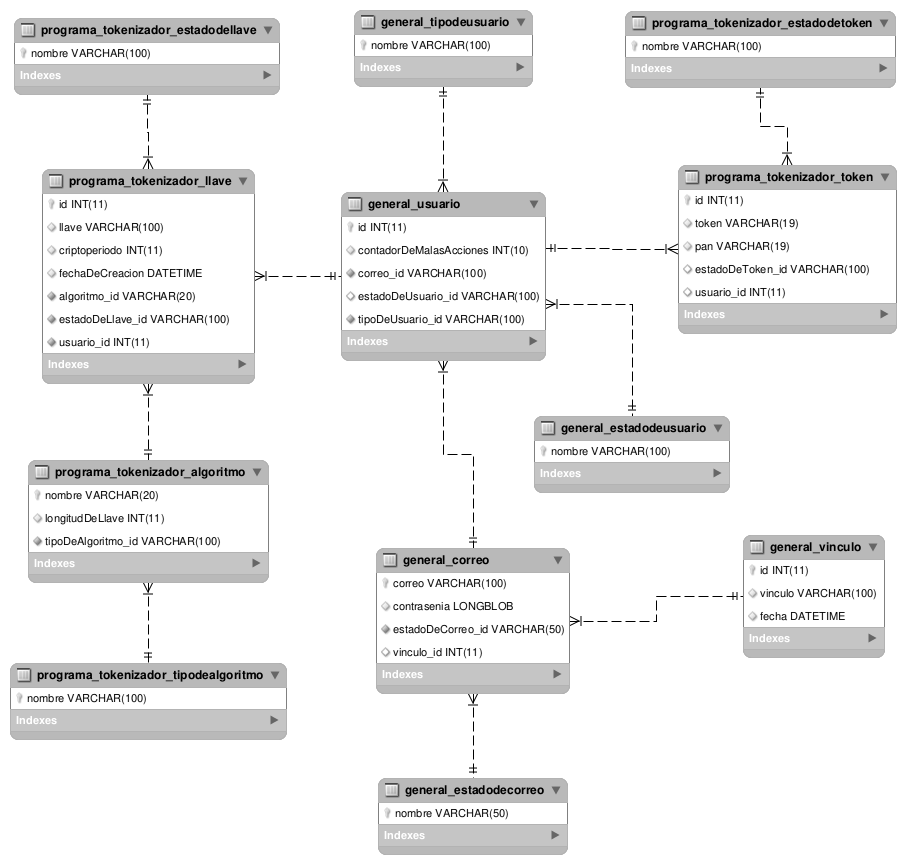
\includegraphics[width=1.0\linewidth]{diagramas/relacional_bn.png}
    \caption{Diagrama relacional de la base de datos.}
    \label{fig:relacional}
  \end{center}
\end{figure}

\subsection{Vista estática}

\begin{sidewaysfigure}
  \begin{center}
    \subimport{diagramas/}{clases.tikz.tex}
    \caption{Diagrama de clases de aplicación web.}
    \label{fig:clases_aplicacion_web}
  \end{center}
\end{sidewaysfigure}

\subsection{Vista dinámica}

En las figuras \ref{fig:secuencia_registrar_cliente} y
\ref{fig:secuencia_tokenizar} se muestran, a modo de ejemplo, diagramas de
secuencia de los casos de uso para registrar un cliente
(\hipervinculo{cu:registrar_cliente}) y para tokenizar un número de tarjeta
(\hipervinculo{cu:tokenizar_tarjeta}); todos los demás casos de uso mantienen
una estructura análoga. En la figura \ref{fig:secuencia_generia} se muestra el
comportamiento dinámico del sistema para las operaciones \gls{gl:crud}.

%
% TODO
% * Hacer que todas las líneas de vida acaben a la misma altura.
% * Poner comentario con hipervínculo a caso de uso.
%

\begin{figure}
  \begin{center}
    \subimport{diagramas/}{secuencia_registrar_cliente.tikz.tex}
    \caption{Diagrama de secuencia para registrar a un cliente.}
    \label{fig:secuencia_registrar_cliente}
  \end{center}
\end{figure}

\begin{figure}
  \begin{center}
    \subimport{diagramas/}{secuencia_tokenizar.tikz.tex}
    \caption{Diagrama de secuencia para operación de tokenización.}
    \label{fig:secuencia_tokenizar}
  \end{center}
\end{figure}

\begin{figure}
  \begin{center}
    \subimport{diagramas/}{secuencia_generica.tikz.tex}
    \caption{Diagrama de secuencia para operaciones genéricas.}
    \label{fig:secuencia_generia}
  \end{center}
\end{figure}
